\documentclass{beamer}
\usepackage{tikz}
\usepackage{fancyvrb}
\title{Centrally Banked Cryptocurrencies\\Security Topics}
\date{November 11, 2016}
\author{Avi Weinstock\\(Paper by George Danezis and Sarah Meiklejohn)}
\begin{document}
\maketitle

% wget 'https://api.blockchain.info/charts/previews/n-transactions-per-block.png?start=1447864475&lang=en&h=405&w=720' -O btc_tx_per_block.png
% https://api.blockchain.info/charts/previews/n-transactions.png?start=1447865253&lang=en&h=405&w=720
% wget 'https://api.blockchain.info/charts/previews/n-transactions.png?start=1447865253&lang=en&h=405&w=720' -O btc_tx_per_day.png
\begin{frame}[fragile]
\frametitle{BTC scalability}
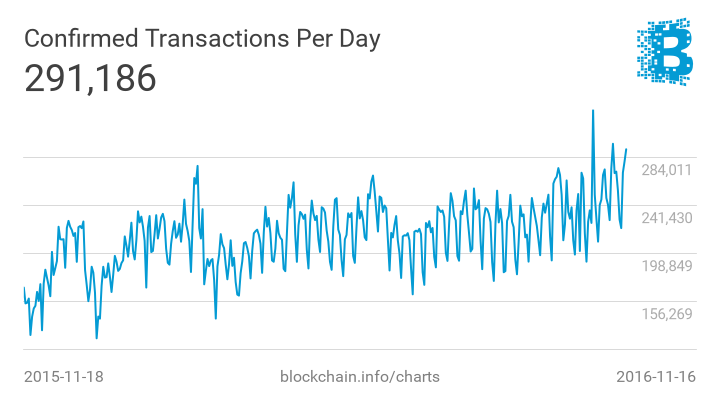
\includegraphics[width=0.9\textwidth]{btc_tx_per_day.png}
\footnote{\Verb|https://api.blockchain.info/charts/previews/n-transactions|\\\Verb|.png?start=1447864475\&lang=en\&h=405\&w=720|}
% >>> 291186.0/(24*60*60)
% 3.3702083333333333
$\frac{291186.0}{24*60*60} \approx 3.3702083333333333$\\
Theoretical max $\frac{\text{transactions}}{\text{second}}$ is 7
\end{frame}

\begin{frame}[fragile]
\frametitle{RSCoin overview}
\begin{itemize}
\item Goal: Create a new cryptocurrency framework that sacrifices decentralized money generation for better performance
\item "Central bank" authorises a large number of "mintettes" to make blocks via PKI
\item Double-spending prevention is still moderately decentralized
\end{itemize}
\end{frame}

\begin{frame}[fragile]
\frametitle{Blockchain hierarchy}
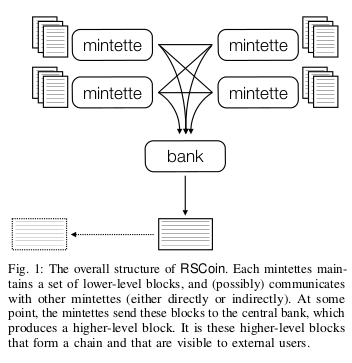
\includegraphics[width=0.9\textwidth]{rscoin_diagram_1.png}
\end{frame}

\begin{frame}[fragile]
\frametitle{Interaction with mintettes}
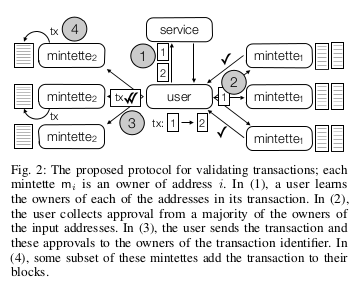
\includegraphics[width=0.9\textwidth]{rscoin_diagram_2.png}
\end{frame}

\begin{frame}[fragile]
\frametitle{Notation (signatures and transactions)}
\begin{itemize}
\item \(
(pk, sk) \leftarrow_\$ \verb|KeyGen|(1^\lambda)\newline
\sigma \leftarrow_\$ \verb|Sign|(sk, m)\newline
\{0,1\} \leftarrow \verb|Verify|(pk, m, \sigma)
\)
\item $\verb|tx| = \{\verb|addr|_i\} \rightarrow^n \{\verb|addr|_j\}$
\item $\verb|addrid| = (\verb|tx|, \verb|index|_{\verb|tx|}(\verb|addr|), v)$
\item $\verb|uxto| : \verb|addrid| \rightarrow \{\bot\} \cup (\verb|addr| \times v)$
\item $\verb|pset| : \verb|addrid| \rightarrow \verb|tx|$
\end{itemize}
\end{frame}

\begin{frame}[fragile]
\frametitle{Notation (high-level blocks)}
High-level blocks (produced by central bank):
\begin{itemize}
\item $B_{\verb|bank|}^i = (h_{\verb|bank|}^i, \verb|txset|_i, \sigma_{\verb|bank|}^i, \verb|DPK|_{i+1})$
\item $h_{\verb|bank|}^i = H(h_{\verb|bank|}^{i-1} || \verb|txset|_i)$
\item $\sigma_{\verb|bank|}^i = \verb|Sign|(sk_{\verb|bank|}, h_{\verb|bank|}^i)$
\end{itemize}
\end{frame}

\begin{frame}[fragile]
\frametitle{Notation (low-level blocks)}
Low-level blocks (produced by mintettes):
\begin{itemize}
\item $\verb|b|_m^j = (h_m^j, \verb|txset|, \sigma, \verb|mset|)\newline$
\item $h_m^j = H(h_{\verb|bank|}^i || h_{j-1}^m || \verb|otherblocks| || \verb|texset|)\newline$
\item $\sigma = \verb|Sign|(sk_m, h)\newline$
\item $\exists \sigma_{\verb|bank|} ((pk_m, \sigma_{\verb|bank|}) \in \verb|DPK|_{i}$
\end{itemize}
\end{frame}

\begin{frame}[fragile]
\frametitle{Sidechains}
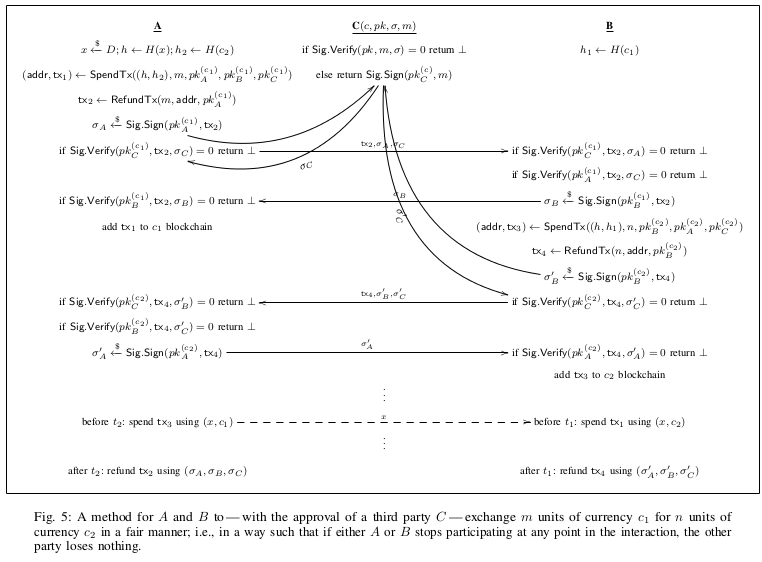
\includegraphics[width=0.9\textwidth]{rscoin_sidechains.png}
\end{frame}

\begin{frame}[fragile]
\frametitle{Resources}
\begin{itemize}
\item "Centrally Banked Cryptocurrencies" by George Danezis and Sarah Meiklejohn \verb|https://eprint.iacr.org/2015/502|
\end{itemize}
\end{frame}
\end{document}
